%# -*- coding: utf-8-unix -*-
% !TEX program = xelatex
% !TEX root = ../thesis.tex
% !TEX encoding = UTF-8 Unicode
%%==================================================
%% chapter02.tex for SJTU Master Thesis
%% based on CASthesis
%% modified by wei.jianwen@gmail.com
%% Encoding: UTF-8
%%==================================================

\chapter{Competition with different updating rules}
\label{chap4}
In this chapter, we control dynamics orders and updating rules for nodes and edges. With changing these updating rules, it is investigated how the states of network are changed. Moreover, it is shown how the updating rules are analyzed in the real world, and which updating rule is more influential for changing a state of the network.\\

\section{Updating rules}

When considering updating rules on two-layer networks, there are many ways to update the state of nodes. Dynamics orders of two layers can be considered whether layer A works first, or layer B works first, or both layers work together. Moreover, orders of nodes can be thought as to whether the states of nodes are changed simultaneously or sequentially or randomly. Orders of edges connected with a node also can be deliberated as to whether edges are activated on a node sequentially or simultaneously or randomly. However, in layer B dynamics, the order of edges in one node always follows the simultaneous updating rule, because dynamics formula already considers the states of all connected neighbor nodes simultaneously. To sum up, as shown in Table~\ref{25updating_rules}, 25 updating rules are considered according to layers, nodes, and edges.

\begin{table}[htp]
	\begin{center}
		\begin{tabular}{c|c|c|c|c}
			Order of layers                                  & \multicolumn{2}{|c|}{Layer A}                                      & Layer B                & remarks   \\ \cline{2-4}
			& Order of nodes                 & Order of edges                     & Order of nodes         &  \\ \hline
			\multirow{10}{*}{Layer A $\rightarrow$ Layer B} & \multirow{4}{*}{Sequential}    & \multirow{2}{*}{Sequential}        & Sequential             & O(o, o) $\to$ D(o) \\  \cline{4-5}  
			&                                &                                    & Simultaneous           & O(o, o) $\to$ D(s) \\  \cline{3-5}     
			&                                & \multirow{2}{*}{Simultaneous}      & Sequential             & O(o, s) $\to$ D(o) \\  \cline{4-5} 
			&                                &                                    & Simultaneous           & O(o, s) $\to$ D(s) \\  \cline{2-5} 
			& \multirow{4}{*}{Simultaneous}  & \multirow{2}{*}{Sequential}        & Sequential             & O(s, o) $\to$ D(o) \\  \cline{4-5}
			&                                &                                    & Simultaneous           & O(s, o) $\to$ D(s) \\  \cline{3-5}
			&                                & \multirow{2}{*}{Simultaneous}      & Sequential             & O(s, s) $\to$ D(o) \\  \cline{4-5}
			&                                &                                    & Simultaneous           & O(s, s) $\to$ D(s) \\  \cline{2-5}
			& \multirow{2}{*}{Random}        & \multirow{2}{*}{Random}            & Sequential             & O(r, r) $\to$ D(o) \\  \cline{4-5}
			&                                &                                    & Simultaneous           & O(r, r) $\to$ D(s) \\   \hline
			\multirow{10}{*}{Layer A $\leftarrow$ Layer B}  & \multirow{4}{*}{Sequential}    & \multirow{2}{*}{Sequential}        & Sequential             & O(o, o) $\leftarrow$ D(o) \\  \cline{4-5}  
			&                                &                                    & Simultaneous           & O(o, o) $\leftarrow$ D(s) \\  \cline{3-5}     
			&                                & \multirow{2}{*}{Simultaneous}      & Sequential             & O(o, s) $\leftarrow$ D(o) \\  \cline{4-5} 
			&                                &                                    & Simultaneous           & O(o, s) $\leftarrow$ D(s) \\  \cline{2-5} 
			& \multirow{4}{*}{Simultaneous}  & \multirow{2}{*}{Sequential}        & Sequential             & O(s, o) $\leftarrow$ D(o) \\  \cline{4-5}
			&                                &                                    & Simultaneous           & O(s, o) $\leftarrow$ D(s) \\  \cline{3-5}
			&                                & \multirow{2}{*}{Simultaneous}      & Sequential             & O(s, s) $\leftarrow$ D(o) \\  \cline{4-5}
			&                                &                                    & Simultaneous           & O(s, s) $\leftarrow$ D(s) \\  \cline{2-5}
			& \multirow{2}{*}{Random}        & \multirow{2}{*}{Random}            & Sequential             & O(r, r) $\leftarrow$ D(o) \\  \cline{4-5}
			&                                &                                    & Simultaneous           & O(r, r) $\leftarrow$ D(s) \\   \hline
			\multirow{2}{*}{Layer A $\leftrightarrow$ Layer B}& \multirow{2}{*}{Simultaneous}& Sequential                         & Simultaneous           & O(s, o) $\leftrightarrow$ D(s) \\ \cline{3-5}
			&                                & Simultaneous                       & Simultaneous           & O(s, s) $\leftrightarrow$ D(s) \\ \hline
			\multirow{3}{*}{Layer A $\Leftrightarrow$ Layer B}& \multirow{2}{*}{Sequential}  & Sequential                         & Sequential             & O(o, o) $\Leftrightarrow$ D(o) \\ \cline{3-5}
			&                                & Simultaneous                       & Sequential             & O(o, s) $\Leftrightarrow$ D(o) \\ \cline{2-5}
			& Random                         & Random                             & Random                 & O(r, r) $\Leftrightarrow$ D(r) \\ \hline
			
		\end{tabular}
	\end{center}
	\caption{25 updating rules according to the order of layers, nodes, and edges}
	\label{25updating_rules}
\end{table}

Updating rules are indicated as follows. `O' and `D'  represent `Opinion layer' and `Decision Making layer' individually. `o' and `s' indicate sequential updating rule and simultaneous updating rule individually. Moreover, the arrow direction indicates the order of layers. In the table remarks, `O(o, o) $\to$ D(s)' represents `Opinion layer(nodes: sequential order updating, edges: sequential order updating) $\to$ Decision-Making layer(node: simultaneous updating)', which means according to the arrow direction, all nodes in the opinion layer are updated with the order of nodes and edges, and then all nodes in the decision-making layer are updated with the order of nodes. `O(o, o) $\Leftrightarrow$ D(o)' means that one node in the opinion layer is updated, and then one node in the decision-making layer is updated until all nodes are updated. Dynamics with 25 updating rules are simulated with the parameters such as $p=0.4$ and $v=0.4$. \\

\section{Competition results}
As the conditions for simulations, each layer consists of the \textit{Barabasi-Albert(BA)} network that has $N$ nodes with attaching new nodes, each with $K$ edges that are preferentially added to existing nodes with a large number of edges as introduced in \parencite{barabasi1999}. Each node of one layer is connected with a random node on the other layer. That means each node has only one external edge. Simulations are performed on the network with $N=2048$ and $K=3$. Simulation results are divided by the order of layers, nodes, and edges.\\

\subsection{Order of layers}
\label{order of layer}
There exist two layers on the interconnected network. Moreover, each layer has its dynamics, such as \textit{M-Model} and \textit{AS-Model}. Two dynamics can be operated simultaneously or sequentially. If two layers act sequentially, the dynamics of layer A can act first, or the dynamics of layer B can work previously. If two layers are operated simultaneously, the order of nodes becomes the simultaneous updating rule automatically because the states of nodes are also changed according to the dynamics of layers. Otherwise, regardless of layers' order, nodes of two layers can interact mutually, i.e., one node in layer A is updated, and then one node in layer B is updated until all nodes are updated. In this case, the order of nodes becomes the sequential updating rule automatically.

There are four ways in order of two layers, \textit{Layer A $\to$ Layer B(sequential), Layer A $\leftarrow$ Layer B(sequential), Layer A $\leftrightarrow$ Layer B(simultaneous), Layer A $\Leftrightarrow$ Layer B(interaction regardless of layers' order)}. 

\begin{figure}[!htb]
	\centering
	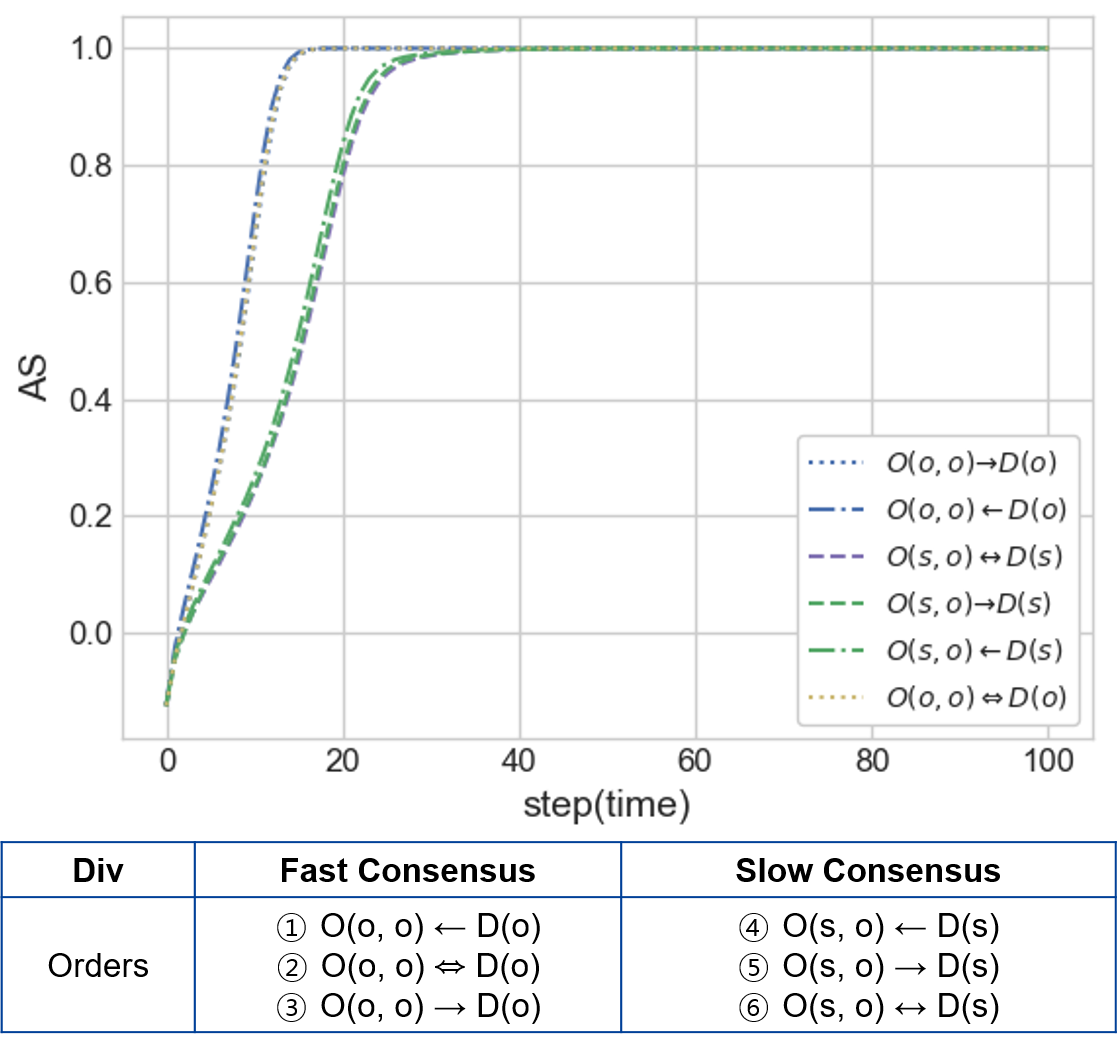
\includegraphics[width=\hsize]{chap4_layerorder.png}
	\caption{Simulation results according to orders of layers: Comparison between orders of layers under the same conditions, such as orders of nodes and edges.}
	\label{chap4_layerorder}
\end{figure}

Fig.~\ref{chap4_layerorder} shows simulation results related to orders of layers. The graph line indicates \textit{AS} value per each step. If the line reaches to $1$ or $-1$, that means the state of the network has a positive or negative consensus state.

As seen in Fig.~\ref{chap4_layerorder}, it is shown that there is little difference according to the orders of layers, but there is a significant difference according to nodes' order. The order of nodes is described in the next subsection~\ref{order of node}. Though consensus time is a little faster when the decision-making layer works first, two orders of layers have almost the same consensus time and result. Regardless of dynamics orders, when other conditions such as updating rules of nodes and edges are the same, the results of the dynamics are also very similar. It is observed that the dynamics order of layers does not have a significant influence on the state of the network. \\

\subsection{Order of nodes}
\label{order of node}
In the simulation models, each layer has $2048$ nodes, and each node has interactions with other nodes. Now, the interaction order of nodes is considered. One node can be updated sequentially after neighbor nodes are updated. Otherwise, every node can be updated simultaneously. Moreover, nodes also can be updated randomly. As the method of random order, one edge is selected randomly and updated until all edges are considered regardless of nodes' orders or edges' orders. (For layer B, random order can not be applied because it has the formula that all edges of a node are considered together) Therefore, simulations are implemented according to three orders of nodes, such as sequential order, simultaneous order, and random order. The interaction orders of nodes can be analyzed as communication methods in the real world. If networks follow a sequential updating rule of nodes, communication methods of networks might be translated as discussion or conversation with enough time. However, if networks follow simultaneous updating rules of nodes, communication methods of networks might be analyzed as vote or election.

\begin{figure}[!htb]
	\centering
	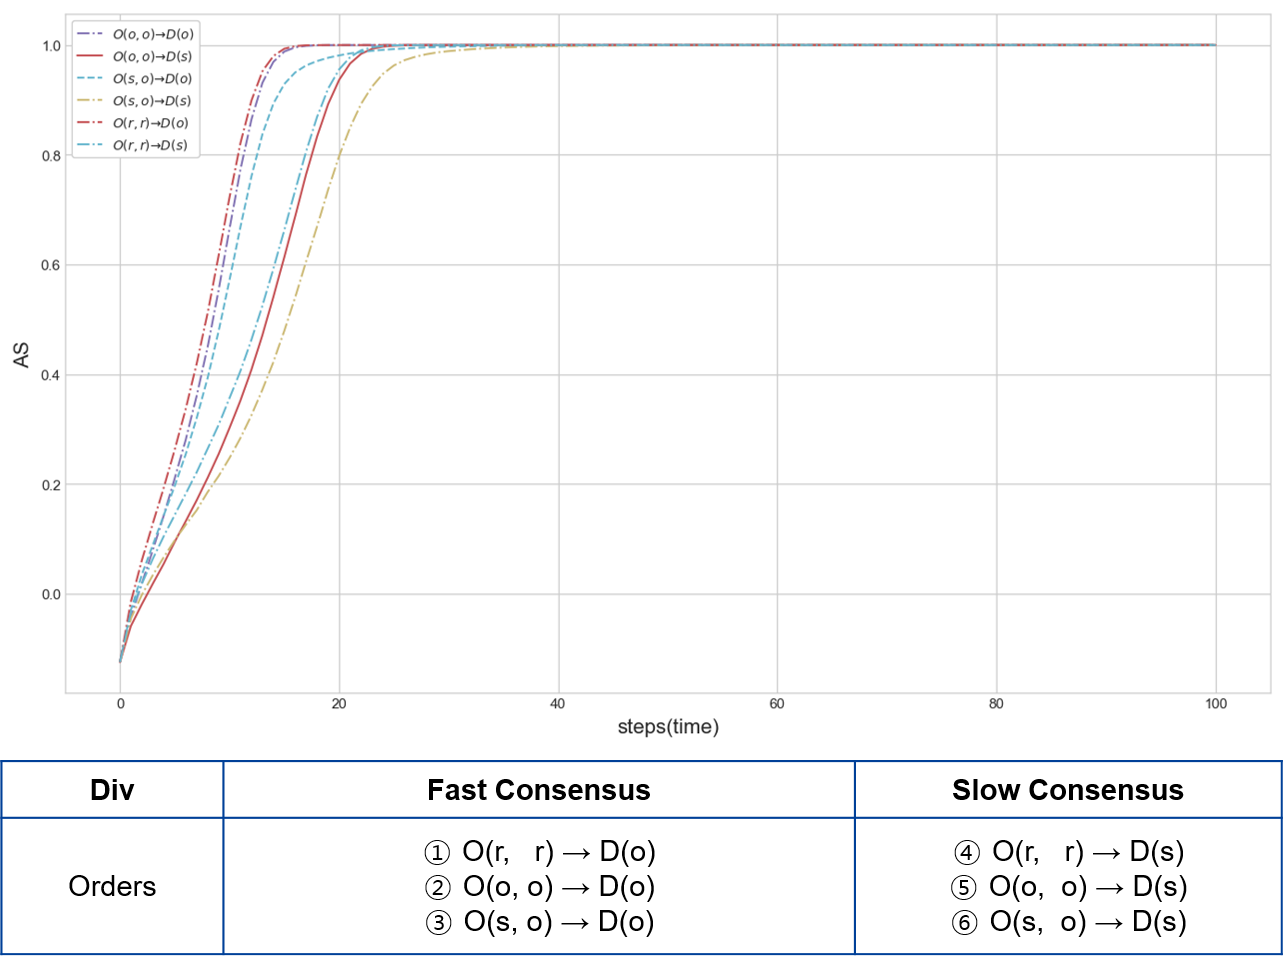
\includegraphics[width=\hsize]{figure/chap4_nodeorder.png}
	\caption{Simulation results according to orders of nodes: Comparison between orders of nodes under the same conditions, such as orders of layers and edges.}
	\label{chap4_nodeorder}
\end{figure}

Fig.~\ref{chap4_nodeorder} shows simulation results according to the interaction orders of nodes. The results are classified into two categories, fast consensus and slow consensus. It is shown that simultaneous interaction between nodes makes a slow consensus. Simultaneous updating rule of nodes in layer A does not make a significant difference with other updating rules of nodes in layer A, but it makes consensus slightly slow. However, simultaneous interaction between nodes in layer B makes consensus much slower than layer A. Random order has similar results with sequential order and does not make different states. 

In conclusion, it is found out that the simultaneous order of nodes makes a slow consensus, and the sequential order of nodes makes a fast consensus. Also, interaction order of nodes in layer B has more influence on consensus time than in layer A. To make quick social consensus, both opinion layer and decision-making layer need sequential updating rule of nodes, such as conversation and discussion.\\     

\subsection{Order of edges}
\label{order of edge}
Each node has several edges connected with other nodes. Updating rules also can be divided according to whether edges are activated sequentially or simultaneously. If the edges work sequentially, a state of the node is changed whenever each edge is activated. Otherwise, if edges of a node are activated simultaneously, a state of the node is changed considering all connected nodes. In the real world, the order of edges in one node can be analyzed as characteristics of nodes. If the order of edges is sequential, the node is analyzed as `rash' because a state of the node is changed whenever edges are activated. If the order of edges is simultaneous, the node is analyzed as `considerate' because it considers all connected nodes together. 

\begin{figure}[!htb]
	\centering
	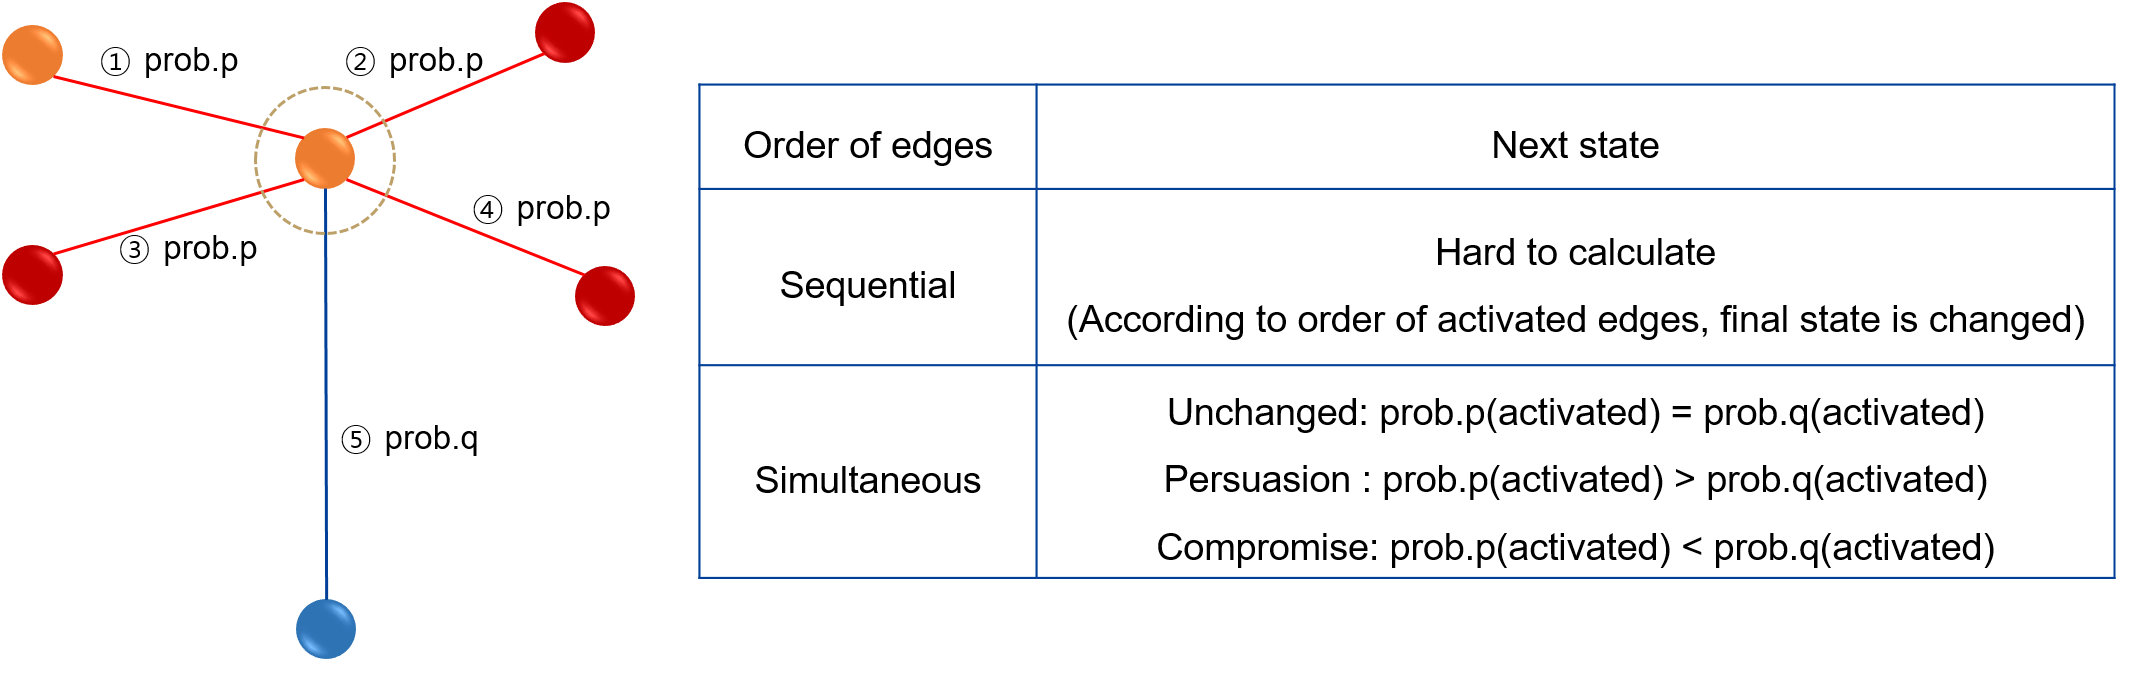
\includegraphics[width=\hsize]{figure/chap4_edgeorder_explanation.png}
	\caption{Order of edges: One node connected with other nodes is updated according to the sequential or simultaneous order of edges}
	\label{edgeorder_explanation}
\end{figure}  

For example, considering the case that one node is connected with other nodes, as shown in Fig.~\ref{edgeorder_explanation}, we can think about how a state of the node is changed according to edges' orders. If the edges follow the sequential updating rule, it is hard to calculate the probabilities because a state of the node is continuously changed according to sequential edges' order. Therefore, the next states of nodes are found out by using computer simulation.

If the edges follow the simultaneous updating rule, it needs some assumptions as follows: 
\begin{enumerate}
	\item If the number of activated \textit{prob.p} is more than the number of activated \textit{prob.q}, persuasion dynamics works. 
	\item If the number of activated \textit{prob.p} is the same as the number of activated \textit{prob.q}, the state is unchanged.
	\item If the number of activated \textit{prob.p} is less than the number of activated \textit{prob.q}, compromise dynamics works.
\end{enumerate}

Through these assumptions, we can calculate probabilities for changing a state of the node by considering all cases as these formulas.  

\begin{equation}
\begin{array}{l}
K = \{ k \quad|\quad 0, \cdots ,{n^{ - {S_i}}}\}, \quad L = \{l \quad|\quad 0, \cdots ,{n^{{S_i}}}\},
\quad M = \{m \quad|\quad k-l\}, \\
{P_A}({S_i} \mapsto {{S'}_i}) = \begin{cases}
\mbox{unchanged}(k = l):\sum {{p^{{n^{ - {S_i}}}+m}} \cdot {{(1 - p)}^{{n^{{S_i}}}-m}} \cdot {}_{{n^{{S_{^i}}}}}{C_k} \cdot {}_{{n^{ - {S_{^i}}}}}{C_l}} \\
\mbox{compromise}(k > l):\sum {{p^{{n^{ - {S_i}}}+m}} \cdot {{(1 - p)}^{{n^{{S_i}}}-m}} \cdot {}_{{n^{{S_{^i}}}}}{C_k} \cdot {}_{{n^{ - {S_{^i}}}}}{C_l}} \\
\mbox{persuasion}(k < l):\sum {{p^{{n^{ - {S_i}}}+m}} \cdot {{(1 - p)}^{{n^{{S_i}}}-m}} \cdot {}_{{n^{{S_{^i}}}}}{C_k} \cdot {}_{{n^{ - {S_{^i}}}}}{C_l}} 
\end{cases}
\end{array}
\label{probabilities}
\end{equation}

In Eq.(\ref{probabilities}), $K$ means the set of an integer from $0$ to the number of nodes with the opposite state(${n^{ - {S_i}}}\}$). $L$ means the set of an integer from $0$ to the number of nodes with the same state(${n^{{S_i}}}\}$). By using permutations and combinations, these formulas are derived.

\begin{figure}[!htb]
	\centering
	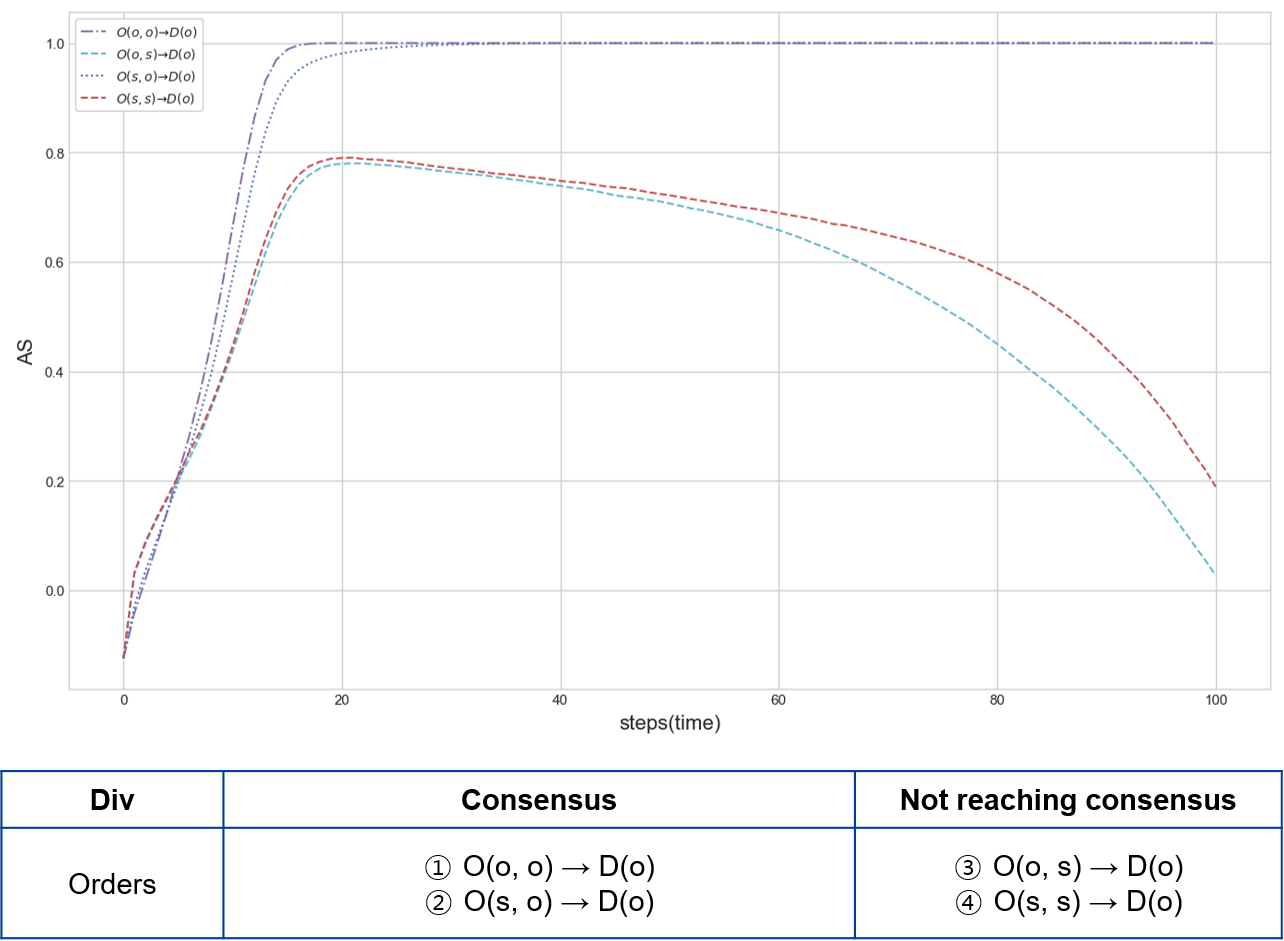
\includegraphics[width=\hsize]{figure/chap4_edgeorder.png}
	\caption{Simulation results according to orders of edges: Comparison between orders of edges under the same conditions, such as orders of layers and nodes}
	\label{edgeorder}
\end{figure}

Fig.~\ref{edgeorder} shows the simulation result according to edges' orders. The results can be categorized into consensus and coexistence(not reaching consensus). The sequential updating rule of edges makes consensus under the same conditions, such as orders of nodes and layers, i.e., rash nodes make consensus. However, the simultaneous updating rule of edges makes it hard to reach consensus under the same conditions, such as orders of nodes and layers, i.e., considerate nodes do not make consensus. It can be analyzed that the rash node is extreme and makes it easy to reach consensus, but the considerate node is moderate and makes it hard to reach consensus.\\
 
\subsection{Comparison and Analysis}
\begin{figure}[!htb]
	\centering
	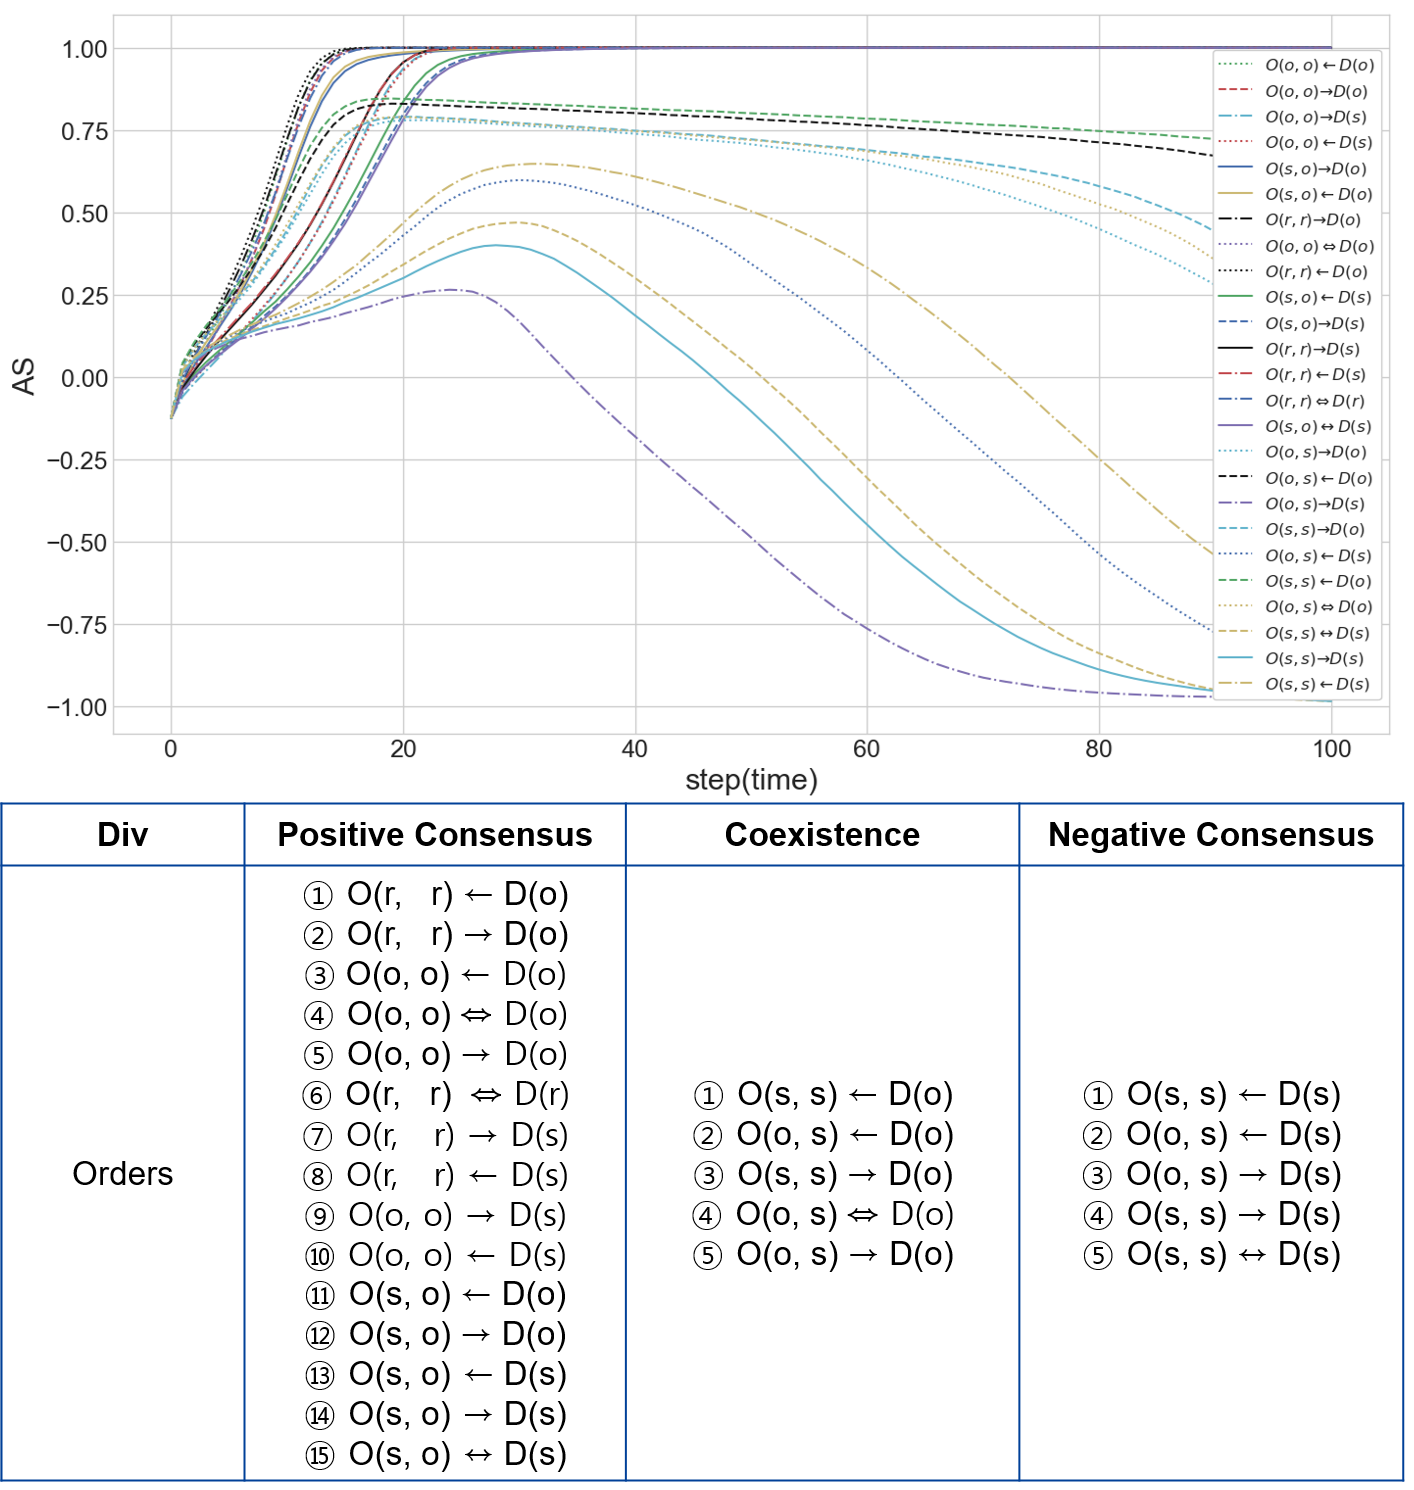
\includegraphics[width=\hsize]{figure/chap4_ordertotal.png}
	\caption{Total results of 25 updating rules with measuring \textit{AS}}
	\label{ordertotal}
\end{figure}

\begin{figure}[!htb]
	\centering
	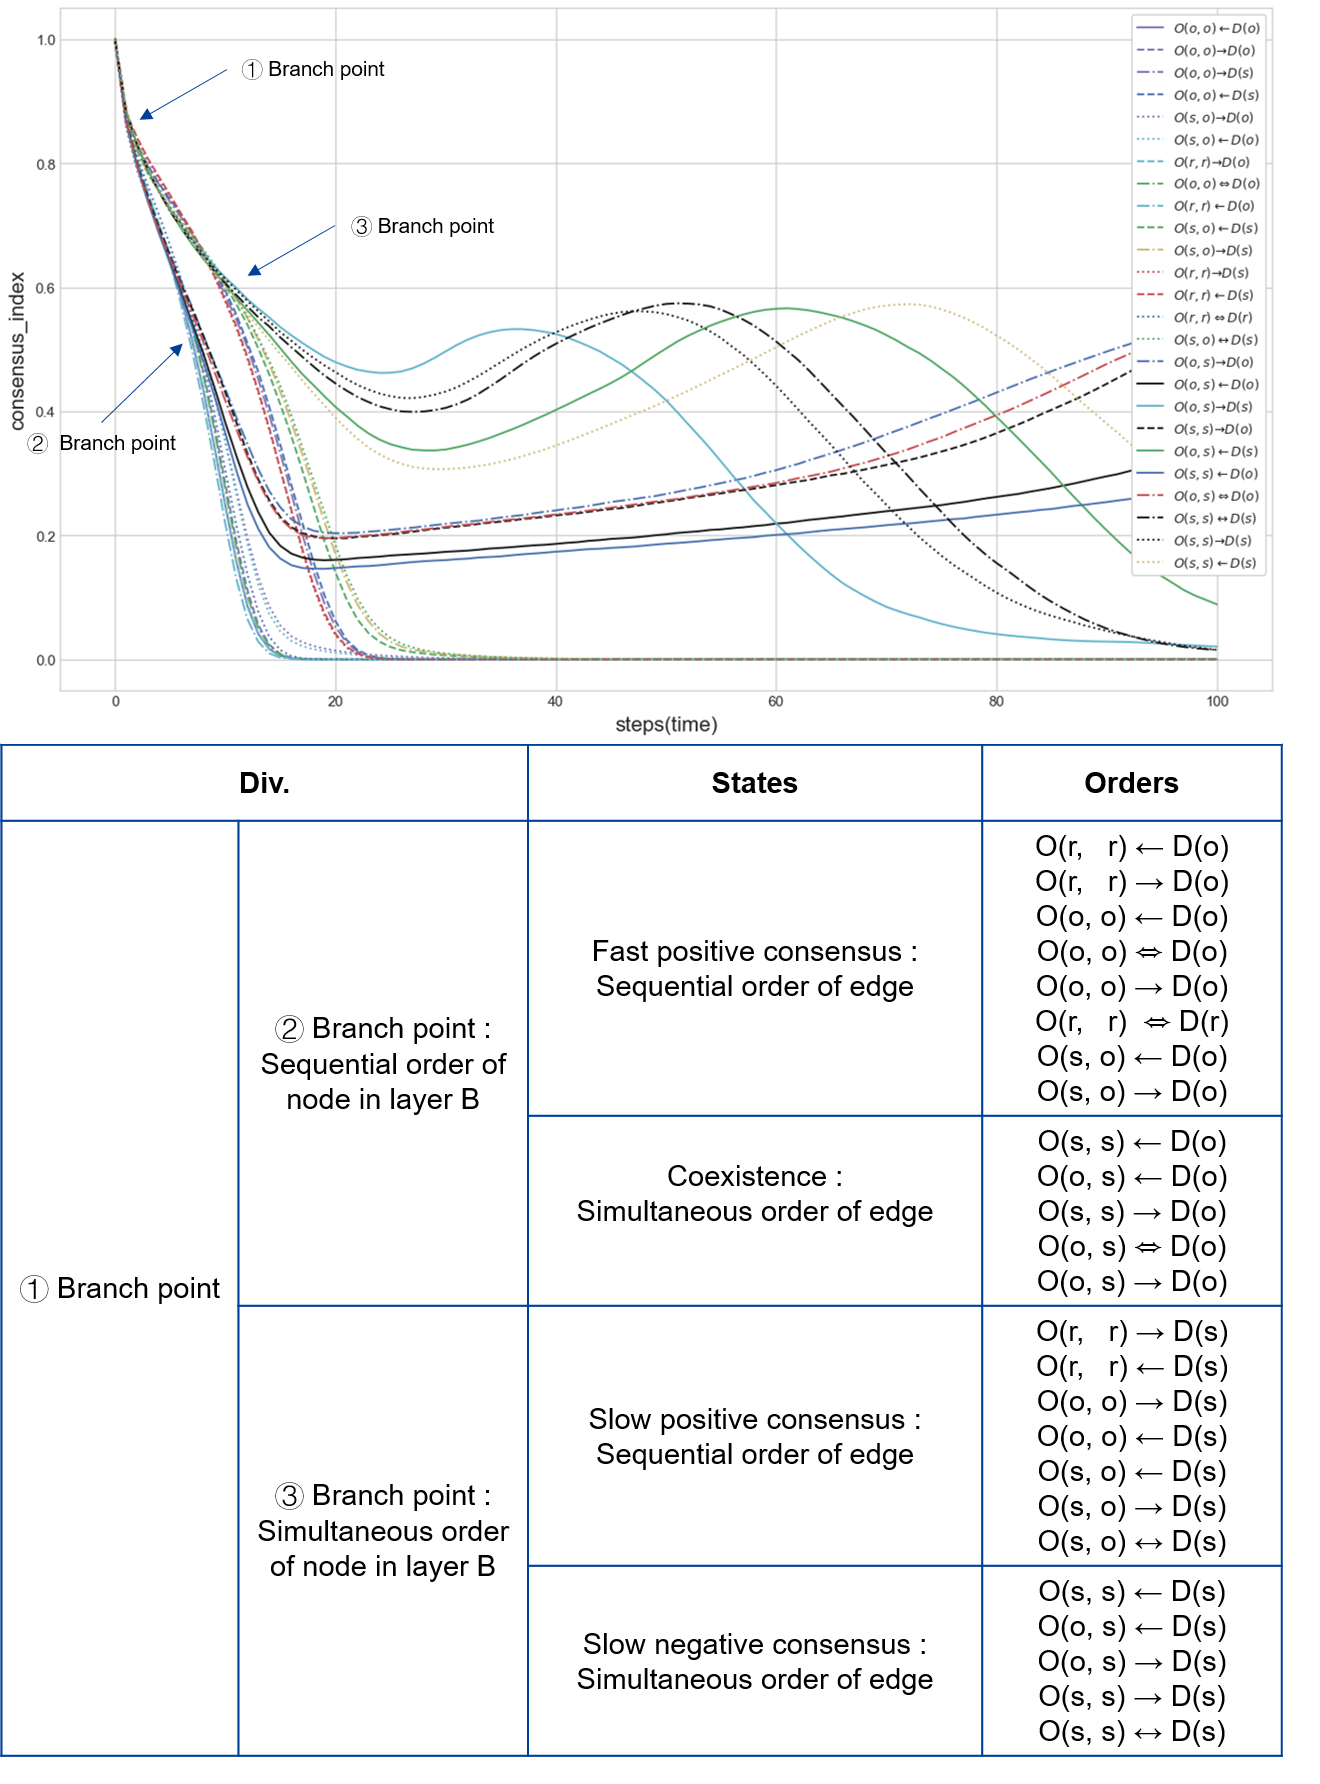
\includegraphics[width=\hsize]{figure/chap4_ordertotal2.png}
	\caption{Total results of 25 updating rules with measuring \textit{CI}}
	\label{ordertotal2}
\end{figure}

It is found out that there are different simulation results according to orders of layers, nodes, and edges. To sum up all updating rules, they can be categorized into three parts, positive consensus, coexistence, and negative consensus, as shown in Fig.~\ref{ordertotal}. 
 
The results can be analyzed by using \textit{CI}, which measures how close the state of the network is to consensus, as shown in Fig.~\ref{ordertotal2}. In this figure, there exist three branch points. In the first branch point, the results are divided according to whether the order of nodes in layer B is sequential or simultaneous. The first branch point makes the results divided into fast opinion convergence and slow opinion convergence. In the second and third branch points, the results are divided according to whether the edges' order in layer A is sequential or simultaneous. The second branch point makes the results divided into consensus and coexistence. The third branch point makes the results divided into positive consensus and negative consensus. To sum up, simulations results are classified into four categories, such as fast positive consensus, slow positive consensus, coexistence, and slow negative consensus. The factors that make branch points have a vital influence on the final state of networks. That means the order of nodes(communication method) in layer B and the order of edges(node characteristics) in layer A have a critical role in determining consensus time and the final state of a network individually. It can be analyzed that the communication method on the decision-making layer makes fast or slow opinion convergence and node characteristics on the opinion layer makes the final state of networks such as positive consensus, negative consensus, and coexistence. \\

\section{Conclusion}
Through these results, several important facts can be arranged. First, networks with simultaneous updating rules tend to make slow consensus or coexistence, sometimes make the transition to opposite orientation. On the other hand, networks with sequential updating rules tend to make fast consensus. Second, dynamics order between layers does not influence network state, though there exists a tiny consensus time gap. Third, the order of nodes in layer B has more influence on network states than the order of nodes in layer A because the order of nodes in layer B makes the first branch point that has a vital role in making fast or slow opinion convergence. That means the communication method in the decision-making layer is very important for determining consensus time. Fourth, the order of edges in layer A is very influential, so that it makes the second and third branch points that determine the final state of the network. It can be analyzed as those characteristics of nodes in layer A, such as `rash' and `considerate', can make the same orientation consensus or make the transition to coexistence or opposite orientation consensus.\\



